\subsection{Protocol Selection}

\subsubsection{Requirements and Options}
\paragraph{Message Requirements}
Table \ref{tab:messages} shows the required messages for flight and imaging. From this it is clear that imaging requires a far higher data transfer speeds. This means a network of low speed modules could be used with a separate imaging network.
\begin{table}[h]
\centering
\begin{tabular}{|c|c|c|c|c|c|c|} 
\hline
\textbf{Protocol} & \textbf{Speed} & \textbf{Complexity} & \textbf{Power Draw} & \textbf{Noise Tolerance} & \textbf{Cost} & \textbf{Use Case} \\ 
\hline 
CAN FD & 5 Mbps & Medium & Medium & High & Medium & Bus \\ 
FlexRay & 10 Mbps & High & High & High & High & Bus \\ 
I$^2$C & 400 Kbps & Low & Low & Low & Low & Sensors \\ 
SPI & 100 Mbps & Medium & Low & Medium & Low & Sensors \\ 
UART & 1 Mbps & Low & Low & Low & Low & Sensors \\ 
Ethernet & 1 Gbps & Medium & Medium & High & Medium & Imaging \\ 
\hline 
\end{tabular}
\caption{Communication Protocols}
\label{tab:communication_options}
\end{table}
\begin{table}[h]
\centering
\begin{tabular}{|c|c|c|c|c|} 
\hline
\textbf{Purpose}&\textbf{Frequency (Hz)}&\textbf{Message Size(bits)}&\textbf{Quantity}&\textbf{Bandwidth (kbps)}\\
\hline
ESC Duty Cycle&400&16&4&25.6\\
ESC Telemetry&10&64&4&2.56\\
Fault ESC Telemetry&400&64&4&102.4\\
Imaging Location&100&48&1&4.8\\
BMS Telemetry&10&32&1&0.32\\
GNSS location&10&48&2&0.96\\
Collision Detection&100&16&2&3.2\\
GNSS Correction&1&500&1&0.5\\
\hline
\end{tabular}
\caption{Required Standard Messages}
\label{tab:device_comms_requirementsl}
\end{table}



\subsubsection{Communication between Modules}
\paragraph{Architecture}
Star architectures consist of a central node directly connected to all the relevant devices, creating a single point of failure on the central node\footnote{\url{hello sailor}}. Federated architectures and distributed architectures, remove this dependency on a single point and therefore represent more complex but more resilient networks\footnote{\url{hello sailor}}. In order to build robustness, the custom \gls{GNSS} module is capable of independently executing landing and \gls{RTS}.  
\paragraph{Bus Selection}
FlexRay has some clear advantages including built in redundancy and higher data transfer speeds\ref{tab:communication_options}. However, due to its added complexity, cost and the fact it is compatible with far fewer components, a \gls{CAN} bus is the better option. This may change if the data transfer rates needed to increase or if the technology behind FlexRay becomes cheaper and more widespread. Further, there are two key options for \gls{CAN}, time triggered or flexible data. Time triggered is an attractive as it supports higher data transfer rates \footnote{\url{hello sailor}} however, flexible data is more widely supported and is sufficient for the application.
\paragraph{CAN bus network}
Devices should be distributed on the lines as in \ref{fig:CAN_bus}, the redundant modules are on separate lines and the modules with no redundancy are connected to both lines. The specific layout is shown in \ref{fig:CAN_bus}.
 \begin{figure}[h!]
 \centering
  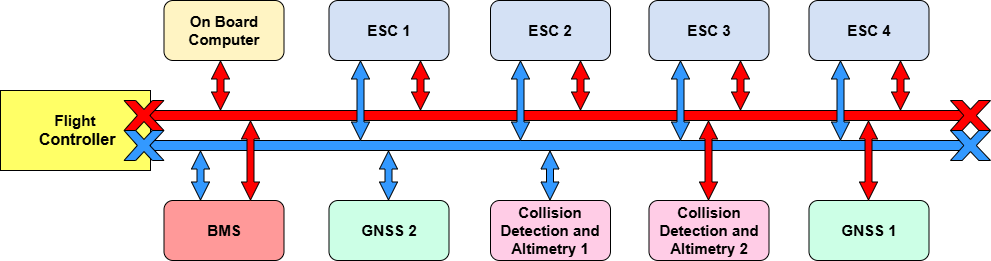
\includegraphics[width=1\textwidth]{figs/Thomas/Intra Communication/CAN bus.png}
 \caption{CAN bus layout}
 \label{fig:CAN_bus}
 \end{figure}
 
\subsubsection{Communication with sensors}
\paragraph{High Speed Sensors}
The simple but high speed \gls{SPI} protocol should be used whenever possible. This is because it is widely supporting by commercially available sensors and \gls{MCU}s \footnote{\url{hello sailor}}. Uniformly using similar sensor sets also has the benefit of simplicity of implementation.
\paragraph{Low Speed Sensors}
Both \gls{UART} and \gls{I$^2$C} are widely supported, both are simple and effective however, \gls{UART} is simpler therefore on non-complex modules is used where possible. However, if pins are limited \gls{I$^2$C} should be used as it can bus multiple low speed sensors.
\paragraph{Memory Devices}
MicroSD and SD cards can communicate with \gls{SPI} or \gls{SDIO}. \gls{SDIO} is the native application and is faster, however, it requires pins that are often more widely distributed on \gls{MCU}s making it more difficult to design with. Therefore, for the flight controller \gls{SPI} was used as the data transfer rates for recording the state vector are low and therefore do not require the higher data transfer rates from \gls{SDIO}. However, while recording imaging data on the main computers SD card, \gls{SDIO} should be used in order to support the ultra high writing speeds required. \textbf{Need a table showing the data transfer rates for telemetry and imaging}
\paragraph{Imaging Sensors}
\textbf{This is a redundant point}
The imaging sensors require very high data transfer rates and are not safety critical. They are therefore not included on the \gls{CAN} bus but instead directly connect to the onboard computer using Ethernet. \textbf{need to mention data transfer rates}
\paragraph{Debugger}
Debugging is possible using the \gls{CAN} bus at a system level but for in depth on board debugging that might be required for failure analysis or uploading code to boards should also be available. This can be done using \gls{UART} however, it is slower and has less functionality than using a \gls{SWD}. \gls{SWD} allows for real-time variable inspection and breakpoints. Therefore, for system wide debugging the \gls{CAN} bus will be used, and for onboard debugging a \gls{SWD} will be used.
\paragraph{High Level Protocol}
A single high level protocol being used across all components makes the \gls{UAV} more adaptable and makes hiring developers easier. This is because a single skill-set can interact with the entire system. Therefore, Cyphal will be used as it can operate over \gls{CAN} and Ethernet \footnote{\url{hello sailor}} which are the key communication systems. 
